\begin{figure}[h]
\begin{center}
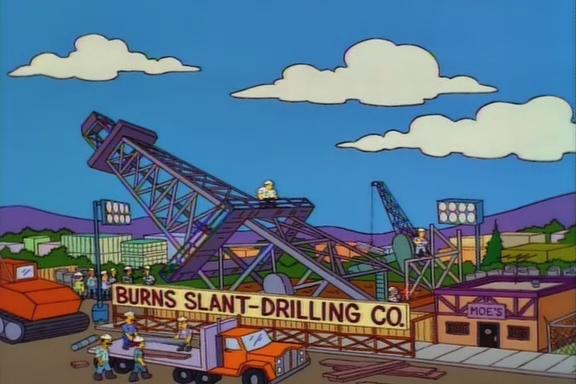
\includegraphics[width=0.6\textwidth] {imagenes/burnsoil.JPG}
\end{center}
\end{figure}

\subsection{Problema a resolver}
El problema a resolver consiste en encontrar un algoritmo que dé un plan de acción para construir una cantidad de refinerías y tuberías entre pozos de petroleo con costo mínimo. Para esto se provee una cantidad de pozos de petroleo, una cantidad de tuberías que se pueden construir entre dos pozos y un costo fijo de poner una refinería en un pozo dado. \\
Se debe encontrar, con el menor costo posible, un plan indicando cuales son las refinerías y tuberías a construir en el que, o bien todas los pozos tengan una refinería, o bien estén conectados a una mediante una o un conjunto de tuberías.

\smallskip
Tenemos los siguientes parámetros de entrada:
	\begin{itemize}[noitemsep,nolistsep]
      \item $n$ = Cantidad de pozos
      \item $m$ = Cantidad de tuberías posibles
      \item $c$ = Costo por refinería
      \item Luego vienen $m$ líneas con tuberías donde $T_{i}$ representa a la tubería en la línea $i$ con $1 \leq i \leq m$ y tiene los siguientes parámetros:
      \begin{itemize}
      \item $o_{i}$ = Tubería de orígen
      \item $d_{i}$ = Tubería de destino
      \item $c_{i}$ = Costo de la tubería
      \end{itemize}
  	\end{itemize}
\smallskip

\subsection{Resolución planteada}
Para resolver este problema, modelaremos la entrada con un grafo, en donde cada pozo es un nodo y cada tubería que podemos construir es una arista con el costo de la construcción de la misma. \\

\begin{itemize}
\item Ejemplo 1:

Sean:
\begin{itemize}
      \item $n$ = 7
      \item $m$ = 6
      \item $c$ = 3
\end{itemize}

Y luego $m$ tuberías:

\begin{table}[H]
\centering
\parbox{0.3\textwidth}{
    \begin{tabular}{ | l | l | l | l |}
    \hline
$T_{i}$ & $o_{i}$ & $d_{i}$ & $c_{i}$ \\ \hline
$T_{1}$ & 1 & 2 & 1 \\ \hline
$T_{2}$ & 3 & 4 & 1 \\ \hline
$T_{3}$ & 2 & 3 & 2 \\ \hline
$T_{4}$ & 1 & 4 & 3 \\ \hline
$T_{5}$ & 5 & 6 & 2 \\ \hline
$T_{6}$ & 2 & 7 & 4 \\ \hline
    \end{tabular}
}
\end{table}

Ésta entrada particular la comprenderíamos con el siguiente grafo:

\tikz[every node/.style={draw,circle}] {
\node (1) at (0, 0)  { 1 };
\node (2) at (2, 0)  { 2 };
\node (3) at (2,-2)  { 3 };
\node (4) at (0,-2)  { 4 };
\node (5) at (4, 0)  { 5 };
\node (6) at (5,-2)  { 6 };
\node (7) at (3,-1)  { 7 };
\draw (1) edge node[above,draw=none] { 1 } (2);
\draw (3) edge node[above,draw=none] { 1 } (4);
\draw (2) edge node[left,draw=none] { 2 } (3);
\draw (1) edge node[left,draw=none] { 3 } (4);
\draw (5) edge node[above,draw=none] { 2 } (6);
\draw (2) edge node[above,draw=none] { 4 } (7);
}

Y una solución válida (no es única) para el siguiente caso se representaría con el siguiente grafo:

\tikz[every node/.style={draw,circle}] {
\node[fill=red!40, text=white] at (3,-1) {7};
\node[fill=red!40, text=white] at (0,0) {1};
\node[fill=red!40, text=white] at (4,0) {5};
\node[fill=blue!40, text=white] at (2,0) {2};
\node[fill=blue!40, text=white] at (2,-2) {3};
\node[fill=blue!40, text=white] at (0,-2) {4};
\node[fill=blue!40, text=white] at (5,-2) {6};
\draw (1) edge[green] node[above,draw=none] { 1 } (2);
\draw (3) edge[green] node[above,draw=none] { 1 } (4);
\draw (2) edge[green] node[left,draw=none] { 2 } (3);
%\draw (1) edge node[left,draw=none] { 3 } (4);
\draw (5) edge[green] node[above,draw=none] { 2 } (6);
%\draw (2) edge node[above,draw=none] { 4 } (7);
}

Donde los nodos rojos representan pozos con refinería, los ejes verdes representan las tuberías que fueron construidas y los nodos azules representan pozos que no tienen una refinería pero están conectadas a una por ejes verdes.
\end{itemize}

Ahora, observemos lo siguiente. Si yo tengo dos pozos unidos por una posible tubería y ésta tiene costo mayor al costo de poner una refinería, entonces esa tubería nunca estará construida en la solución.
Por ejemplo:
\begin{itemize}
\item Ejemplo 2:

Sean:
\begin{itemize}
      \item $n$ = 2
      \item $m$ = 1
      \item $c$ = 3
\end{itemize}

Y luego $m$ tuberías:

\begin{table}[H]
\centering
\parbox{0.3\textwidth}{
    \begin{tabular}{ | l | l | l | l |}
    \hline
$T_{i}$ & $o_{i}$ & $d_{i}$ & $c_{i}$ \\ \hline
$T_{1}$ & 1 & 2 & 5 \\ \hline
    \end{tabular}
}
\end{table}

Esta entrada particular la comprenderíamos con el siguiente grafo:

\tikz[every node/.style={draw,circle}] {
\node (1) at (0, 0)  { 1 };
\node (2) at (2, 0)  { 2 };
\draw (1) edge node[above,draw=none] { 5 } (2);
}

En este caso, construyendo la tubería, el grafo solución sería el siguiente:

\tikz[every node/.style={draw,circle}] {
\node[fill=red!40, text=white] at (0,0) {1};
\node[fill=blue!40, text=white] at (2,0) {2};
\draw (1) edge[green] node[above,draw=none] { 5 } (2);
}

Acá tendríamos un costo total de 8 (una refinería con costo 3 más la tubería con costo 5).

Sin embargo,la solución correcta sería la siguiente:

\tikz[every node/.style={draw,circle}] {
\node[fill=red!40, text=white] at (0,0) {1};
\node[fill=red!40, text=white] at (2,0) {2};
}

Donde el costo total sería 6 (dos refinerías de costo 3)
\end{itemize}



Y esto lo podemos generalizar: \\

\begin{lemma}
        sean dos componentes conexas $C_{1}$ y $C_{2}$ con las tuberías necesarias construidas para garantizar un costo mínimo, y sea $T$ una posible tubería entre un pozo en $C_{1}$ y uno en $C_{2}$. $T$ solo será construída en una solución de costo mínimo si su costo es menor o igual al costo de la refinería.
    \end{lemma}

\begin{proof}
Sea $costo()$ la función que recibe un conjunto de pozos y tuberías construidas y devuelve el costo total de la construcción. \\

Sea $c$ el costo de una refinería.

Una componente conexa que está en una solución válida tiene costo mínimo, por ende, sólo tiene una refinería en ella porque en caso de tener un pozo que este conectado a una refinería por tuberías, y que a su vez tenga una refinería en el pozo, ésta no sería una solución mínima ya que puedo eliminar esa refinería reduciendo el costo total y el pozo seguiría estando conectado con una.

Ahora, sean dos componentes conexas $C_{1}$ y $C_{2}$ con las tuberías necesarias construidas para garantizar un costo mínimo, y sea $T$ una posible tubería entre un pozo en $C_{1}$ y uno en $C_{2}$.

El costo de la tubería $T$ es $costo(T)$.

Mi costo acumulado de $C_{1}$ y $C_{2}$ es $costo(C_{1})$ y $costo(C_{2})$ respectivamente.

Como estamos buscando minimizar el costo, $T$ debe ser construida si se da lo siguiente:

$$costo(C_{1}) + costo(C_{2}) \geq costo(C_{1}) + costo(C_{2}) + costo(T) - c$$

Entonces, despejando, solo debe ser construida si:

$$c \geq costo(T)$$
\end{proof}

Por lo tanto, ya que una tubería con costo mayor al de una refinería nunca va a ser construida, podríamos no agregarla al modelar la entrada en un grafo. En el ejemplo 1, el grafo quedaría de la siguiente manera:

\tikz[every node/.style={draw,circle}] {
\node (1) at (0, 0)  { 1 };
\node (2) at (2, 0)  { 2 };
\node (3) at (2,-2)  { 3 };
\node (4) at (0,-2)  { 4 };
\node (5) at (4, 0)  { 5 };
\node (6) at (5,-2)  { 6 };
\node (7) at (3,-1)  { 7 };
\draw (1) edge node[above,draw=none] { 1 } (2);
\draw (3) edge node[above,draw=none] { 1 } (4);
\draw (2) edge node[left,draw=none] { 2 } (3);
\draw (1) edge node[left,draw=none] { 3 } (4);
\draw (5) edge node[above,draw=none] { 2 } (6);
}

Entonces, de ahora en adelante modelaremos la entrada en un grafo, pero solo añadiremos como aristas las tuberías que tengan costo menor al costo de la refinería. \\

Notemos que podemos dividir nuestro problema en un subproblema por cada componente conexa que tenga nuestra entrada. \\

Necesitamos entonces, encontrar una solución mínima en cada componente conexa. Notemos ahora que si una componente conexa está en el modelo, entonces existe una solución con una sola refinería para toda la componente, ya que se puede llegar de cualquier pozo a cualquier otro mediante tuberías posibles y que todas las tuberías tienen costo menor al costo de una refinería. Notemos también que la solución no tendrá ciclos, ya que de tenerlos, ésta solución no sería mínima porque se podría eliminar una tubería perteneciente al ciclo, reduciendo el costo total de la construcción y aún así se podría llegar de cualquier nodo de la componente a cualquier otro mediante tuberías. \\

Sacando en limpio estos datos, lo que estamos buscando en cada componente es encontrar una solución que recorra todos los nodos de la componente, es decir, que sea conexa, que no tenga ciclos, y que a la vez tenga costo mínimo. Entonces, lo que estamos buscando es encontrar el árbol generador mínimo de cada componente conexa. \\

Ahora, si encuentro un árbol generador mínimo de cada componente conexa del grafo con el que modelamos la entrada, estaría consiguiendo una solución con costo mínimo. Entonces, lo que el problema realmente nos está pidiendo es encontrar un bosque generador mínimo del grafo, ya que debemos minimizar los costos de la construcción de refinerías y tuberías. \\

Para resolver el siguiente problema, usaremos el algoritmo de Kruskal. \\
Dado un grafo, el algoritmo de Kruskal se encarga de encontrar el árbol generador mínimo en el mismo, y en caso de no ser posible porque el grafo tiene más de una componente conexa, el algoritmo encuentra el bosque generador mínimo. \\
\\
El algoritmo de Kruskal, ordena primero las aristas del grafo según su costo en una estructura y luego recorre la misma en orden fijándose por cada arista si los dos nodos pertenecen a la misma componente, si estos no pertenecen a la misma componente, agrega la arista y une las componentes, y si pertenecen a la misma componente desestima esa arista ya que ya están conectadas. \\
\\
De esta forma, al finalizar de recorrer la estructura quedarían tantos árboles como componentes conexas tiene el grafo, como estos árboles tienen costo mínimo, el bosque resultante es el bosque generador mínimo.  \\
\\
En nuestro caso, usaremos como estructura una cola de prioridad que priorice por menor costo. Además, para modelar el grafo correctamente, solo añadiremos a la cola de prioridad las tuberías posibles que tengan costo menor al costo de construir una refinería.


\subsubsection{Pseudocódigo}

Pseudocódigo de la solución

\begin{codesnippet}
//Creamos un entero con el costo de crear una refinería en cada pozo
int costoTotal <- n*m

//Creo una cola de prioridad
ColaPrior tuberías

//Sea t el conjunto con las tuberías que se reciben en el input
//Encolamos en la cola de prioridad las tuberías de t con costo menor a c
Por cada tubería i de las m posibles que se ingresan en t
	Si el costo de la tubería i es menor a c
    	tuberías.encolar(t[i])
    Fin si
Fin por

//Creamos un vector de tuberías donde guardare las tuberías que se construyen
Vector tuberíasConstruidas

//Creamos un conjunto disjunto con los pozos
UnionFind componentes(n)

Mientras tuberías no este vacío
  //Sea top el primer elemento de la colaPrior tuberías
  	top <- tuberías.primero()

    Si el origen de la tuberías top no esta en el mismo conjunto que el destino
      //Unimos los conjuntos a los que pertenecen ambos pozos
        componentes.unir(top.origen,top.destino)

        //Agregamos a top al vector de tuberías construidas
        tuberíasConstruidas.agregarAtras(top)

        //Bajamos el costo total
        costoTotal <- costoTotal - c + top.costo
    Fin si

    //Desencolamos a top de la cola de prioridad
    tuberías.desencolar()
Fin mientras

//Ahora solo resta mostrar la solución
Mostramos costoTotal, la cantidad de conjuntos que tiene componentes y
el tamaño de tuberíasConstruidas

//Mostramos un elemento de cada conjunto de componentes
Por cada conjunto en componentes
	mostrar el primer elemento
Fin por

//Mostramos las tuberías construidas
Por cada tubería i en tuberíasConstruidas
	mostrar tuberíasConstruidas[i]
Fin por
\end{codesnippet}
Pseudocódigo de la estructura UnionFind: \\

\begin{codesnippet}
Vamos a representar cada conjunto como un árbol.
Tengo dos arreglos de tamaño n, uno que representa el id al que pertenece el elemento i,
con i entre 0 y n. Y el otro representa el rank del elemento i.
El id lo que indica es quien es la raíz del árbol al que pertenece el elemento.
A la vez, tengo un entero llamado cantidadDeArboles que tiene tamaño n al inicializar.

//devuelve la raiz del arbol a la que pertenece un elemento
buscar(p)
  raiz = p
  mientras raiz != id[raiz]
  	raiz = id[raiz]
  mientras p != raiz
  	newp = id[p]
  	id[p] = raiz
  	p = newp

  return raiz

//une dos componentes
unir(x, y)
  i = buscar(x)
  j = buscar(y)

  //si son iguales ya estaban en la misma componente
  si i == j return

  //hace que la raiz del menor apunte a la del mayor
  si rank[i] < rank[j]
    id[i] = j
  sino
   id[j] = i
   si rank[i] == rank[j]
    rank[i]++;


  cantidadDeArboles--;


//devuelve true si dos elementos estan en el mismo arbol
conectados(x,y)
   return buscar(x) == buscar(y);


count()
	return cantidadDeArboles;

\end{codesnippet}



\subsection{Complejidad propuesta}

Como se ve en el pseudocódigo, la solución al problema se divide en tres partes, que son guardar los datos de entrada, encontrar la solución y mostrarla. El enunciado nos pide resolver todo en una complejidad estrictamente menor a  $\mathcal{O}(n^{3})$. \\

Al procesar la entrada, se guardan $n$, $m$ y $c$ en $\mathcal{O}(1)$, se crea un UnionFind con n conjuntos en $\mathcal{O}(n)$, y luego se guardan las tuberías posibles con costo menor a $c$ en una cola de prioridad. Las tuberías son a lo sumo $m$ y encolar cada una tiene costo $\mathcal{O}(log(m))$. Por lo tanto, todo el proceso de guardar los datos de entrada tiene complejidad $\mathcal{O}(m*log(m))$, y como $m$ está acotado superiormente por $n^2$, la complejidad sería $\mathcal{O}(n^2*log(n))$. \\

Veamos ahora la complejidad de encontrar la menor solución. Esto se realiza en un ciclo definido por el tamaño de la cola de prioridad, que es a lo sumo $m$. Dentro del ciclo, se guarda el primer elemento de la cola, esto se realiza en $\mathcal{O}(1)$. Luego se revisa si ambas tuberías pertenecen al mismo conjunto del UnionFind, de no ser así, estas se unen. \\

Entonces, por cada tubería, tengo a lo sumo que llamar dos veces a la función buscar y una vez a la función unir del UnionFind. \\

Si la tubería es construida, además de unir en el UnionFind, se debe agregarla al vector que guarda las tuberías construidas, y esto se hace en $\mathcal{O}(1)$. También, se debe bajar el costo total de la construcción que también es $\mathcal{O}(1)$.

Como podemos ver en el pseudocódigo, nuestro UnionFind utiliza las dos heurísticas para UnionFind implementado sobre árboles. Éstas son union by rank y path compression.

La heurística path compression está implementada en la función buscar y lo que hace es que al buscar un elemento, les actualiza no solo a el elemento sino a todos sus padres la raíz a la raíz del árbol. Esto hace que en llamados posteriores no sea necesario recorrer todo el árbol.

La heurística union by rank para cada x, define rank[x] como alguna
cota superior para la altura del subarbol con raíz en x y luego hace la unión por el tamaño de rank. Esto hace que la unión sea $\mathcal{O}(\log(n))$ porque cada conjunto tiene a lo sumo n elementos y el rank de un árbol sube solo al unirlo con otro de su mismo tamaño. \\

Combinando estas dos heurísticas, nos queda una complejidad total de encontrar la mejor solución de $\mathcal{O}(m*\alpha(n))$\footnote{La demostración se encuentra en Thomas H. Cormen, Charles E. Leiserson, Ronald L. Rivest, and Clifford Stein. Introduction to Algorithms.
The MIT Press, 2001.}
donde $\alpha$ es el inverso de la función de Ackermann y está acotado por 5 para todo uso práctico. Ahora, como $m$ está acotado superiormente por $n^2$, la complejidad sería $\mathcal{O}(n^2*\alpha(n))$, y en particular, está acotado por $\mathcal{O}(n^2*log(n))$.\\


Luego resta la parte de mostrar la solución, esto se hace en $\mathcal{O}(1)$ para mostrar el costo total, la cantidad de refinerías construidas y la cantidad de tuberías construidas. Se muestran en $\mathcal{O}(m) = \mathcal{O}(n^2)$ todas las tuberías que fueron construidas, ya que hay que recorrer el vector de tuberías. Y, por último, se realiza un ciclo que, por cada pozo, muestra el pozo si tiene una refinería en el mismo. Vamos a decir que un pozo tiene una refinería si es la raiz del árbol al que pertenece en el UnionFind. Entonces, si acotamos el buscar del UnionFind por $\mathcal{O}(\log(n))$ ya que el árbol está balanceado, tenemos una complejidad de $\mathcal{O}(m*\log(n))$, y como $m$ está acotado superiormente por $n^2$, la complejidad sería $\mathcal{O}(n^2*log(n))$. \\

Por lo tanto, sumando todas las étapas de la solución, nos quedaría:

$$\mathcal{O}(n^2*log(n)) + \mathcal{O}(n^2*\alpha(n)) + \mathcal{O}(n^2) + \mathcal{O}(n^2*log(n))$$

O sea,

$$\mathcal{O}(2*n^2*log(n) + n^2*\alpha(n) +(n^2) \in \mathcal{O}(n^2*log(n)) $$

Por lo tanto, nuestra complejidad teoríca final es
$$\mathcal{O}(n^2*log(n))$$

Y ésta es estrictamente menor a  $\mathcal{O}(n^3)$ como pedía el enunciado.

\newpage
\subsection{Implementación en C++}
\lstinputlisting[language=C++, breaklines]{codigo/ej3.cpp}

\newpage
\subsection{Experimentación computacional}
La función que utilizamos para llevar a cabo las mediciones fue \texttt{std::clock}\footnote{Referencia \url{http://en.cppreference.com/w/cpp/chrono/c/clock}}. La unidad temporal que utilizamos para este ejercicio fue milisegundos.
La complejidad teórica calculada es de $\mathcal{O}(n^2* \log(n))$


\subsubsection{Experimentación con instancias aleatorias}
Para generar las instancias aleatorias utilizamos la función \texttt{std::rand}\footnote{Referencia \url{http://en.cppreference.com/w/cpp/numeric/random/rand}} con determinados intervalos de valores para la variables, para obtener instancias coherentes. El detalle de intervalos es el siguiente:
\begin{itemize}
	\item Cantidad de pozos ($n$): 2 $\leq n \leq$ 1000
    \item Cantidad de tuberías ($m$): 1 $\leq m \leq \frac{n(n-1)}{2}$
    \item Costo de refinería ($c$): 1 $\leq c \leq$ 1000
\end{itemize}

No se generaron muestras para n = 1 ya que no hay tuberías posibles.
Generamos 20 instancias aleatorias para cada $n$, variando aleatoriamente el $m$ y el $c$ en cada muestra y luego fueron promediadas. Su medición temporal, arroja el siguiente resultado:


\begin{figure}[H]
        \centering
\begin{subfigure}[b]{0.5\textwidth}
                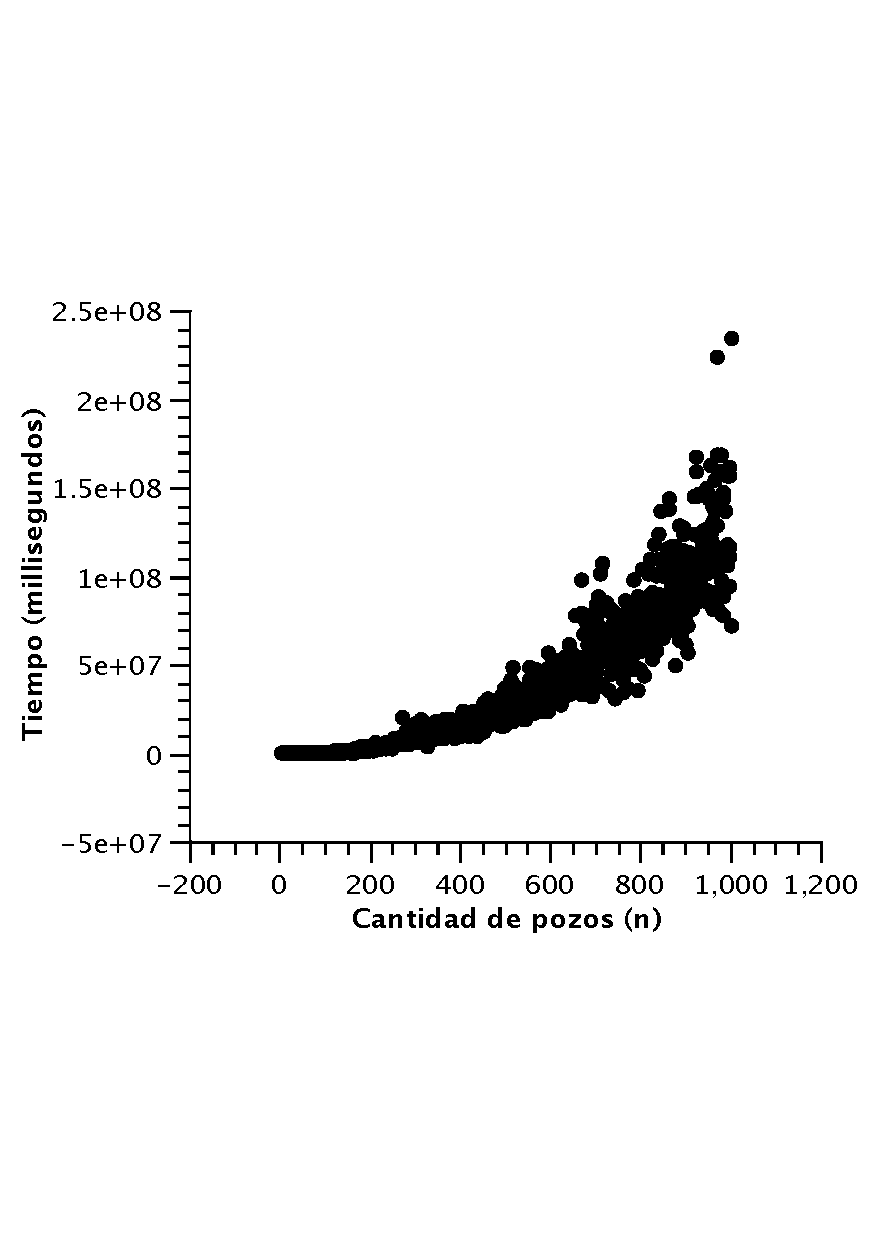
\includegraphics[width=\textwidth]{imagenes/ej3-rawData.pdf}
                \caption*{Tiempos sin procesar, en milisegundos}
        \end{subfigure}%

        \begin{subfigure}[b]{0.5\textwidth}
                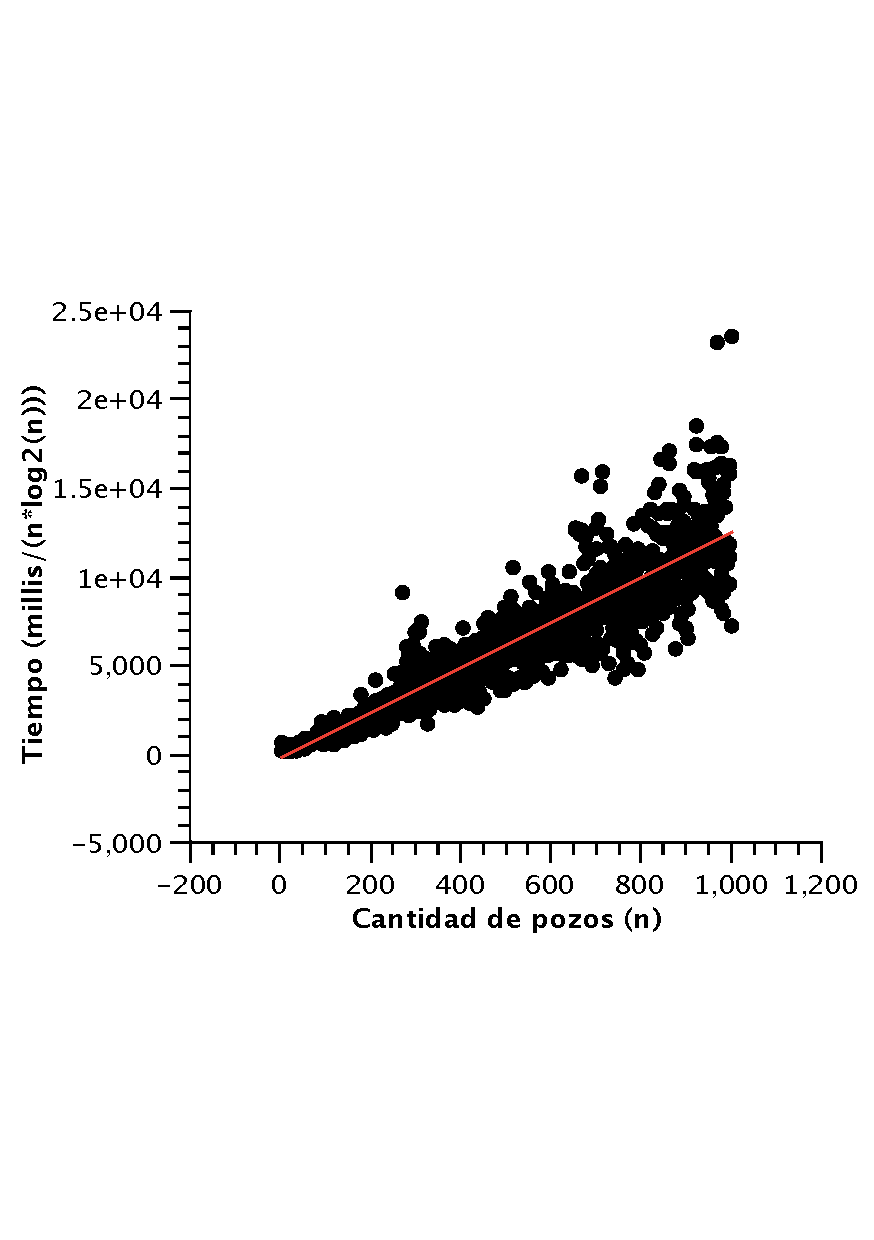
\includegraphics[width=\textwidth]{imagenes/ej3-nlogn.pdf}
                \caption*{Dividiendo a los tiempos por $n \log(n)$}
        \end{subfigure}

\end{figure}

\begin{figure}[H]
        \centering

        \begin{subfigure}[b]{0.5\textwidth}
                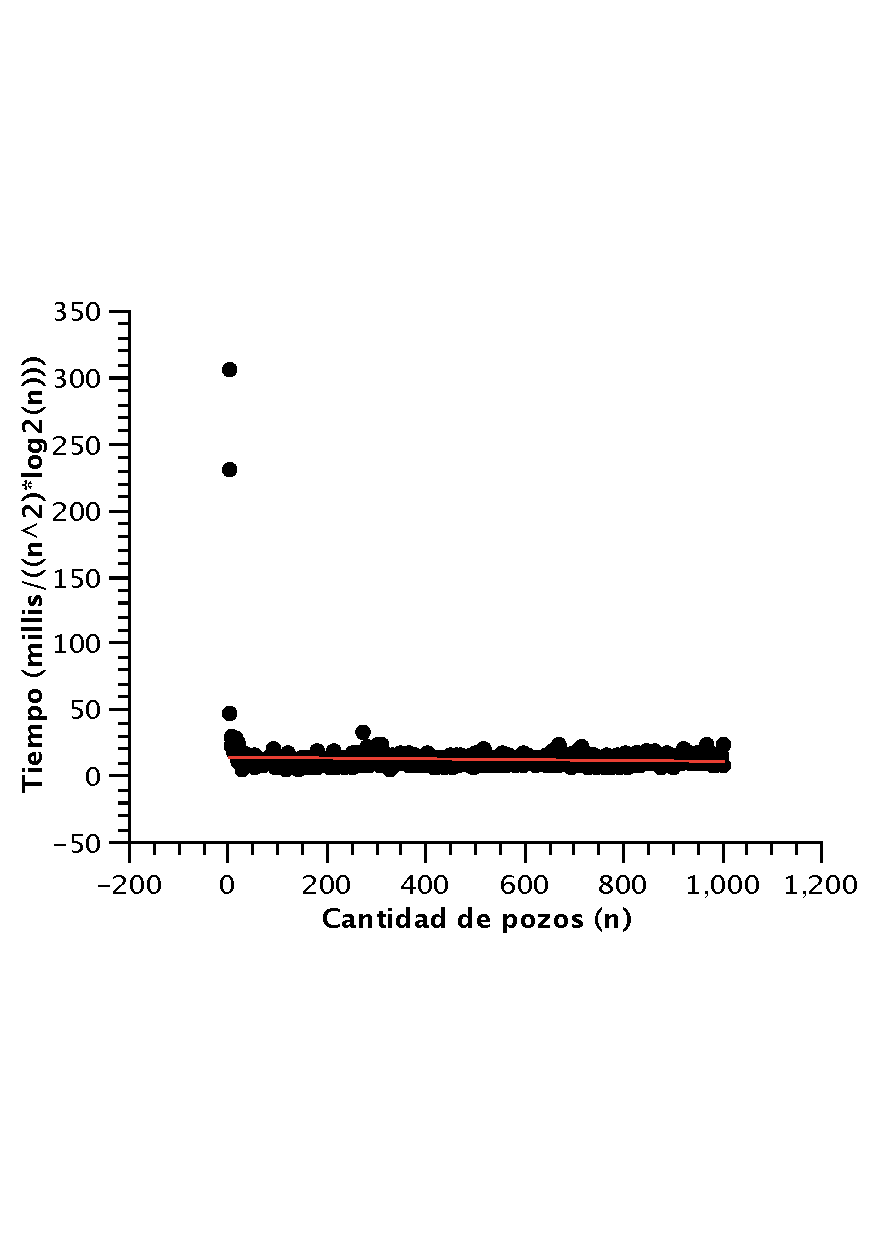
\includegraphics[width=\textwidth]{imagenes/ej3-const.pdf}
                \caption*{Dividiendo a los tiempos por $n^2 \log(n)$}
        \end{subfigure}

\end{figure}


A continuación, adjuntamos una tabla con los últimos 20 valores obtenidos en las instancias aleatorias, teniendo en cuenta que los casos fueron previamente ordenados según el tamaño ($n$):

\begin{table}[H]
\parbox{0.3\textwidth}{
    \begin{tabular}{ | l | l | l | l |}
    \hline
n   &Tiempo(milisegundos) &Tiempo(mili/($n^2 \log(n)$)) &Tiempo(mili/($n \log(n)$)))\\ \hline
980	&106,884,913.7		&11.20017462183745	&10,976.17112940071\\ \hline
981	&148,013,000.5		&15.47597708270933	&15,181.93351813786\\ \hline
982	&143,649,318.15		&14.98692707630785	&14,717.16238893431\\ \hline
983	&88,530,761.25		&9.21626618012942	&9,059.589655067221\\ \hline
984	&77,926,122.55		&8.09462319280639	&7,965.109221721488\\ \hline
985	&96,363,820.55		&9.98806386893941	&9,838.242910905317\\ \hline
986	&137,058,449.3		&14.17515494504867	&13,976.70277581799\\ \hline
987	&109,314,001.3		&11.28115224428363	&11,134.49726510795\\ \hline
988	&116,393,678.25		&11.98570806428229	&11,841.8795675109\\ \hline
989	&95,277,182.2		&9.789957451616216	&9,682.267919648439\\ \hline
990	&106,078,816.3		&10.87624855027109	&10,767.48606476838\\ \hline
991	&156,976,954.55		&16.0600124239817	&15,915.47231216586\\ \hline
992	&112,528,406.3		&11.48768775240836	&11,395.7862503891\\ \hline
993	&117,798,450.6		&11.99972974500853	&11,915.73163679347\\ \hline
994	&109,700,234.25		&11.1506922114351	&11,083.78805816649\\ \hline
995	&156,578,939.15		&15.88147949436476	&15,802.07209689294\\ \hline
996	&117,020,018.95 	&11.84355454694666	&11,796.18032875887\\ \hline
997	&94,736,198.95		&9.567601826537732	&9,538.89902105812\\ \hline
998	&161,853,906.15 	&16.31084667818704	&16,278.22498483067\\ \hline
999	&110,925,527.35		&11.15454731027924	&11,143.39276296896\\ \hline
1,000	&72,523,403.45		&7.27723994203022	&7,277.239942030219\\ \hline
    \end{tabular}
}
\end{table}


Como podemos ver de los gráficos y la tabla suministrada,al dividir los tiempos por $n* \log(n)$, tienden a algo lineal, mientras que al dividir los tiempos por $n^2* \log(n)$, tienden a un número constante. Entonces nuestro algoritmo tendría complejidad $\mathcal{O}(c*n^2* \log(n))$, donde $c$ es la constante a la cual converge el gráfico. Por lo tanto concluimos que los gráficos se condicen con nuestra predicción de complejidad.


\subsubsection{Experimentación con instancias particulares}

Para este problema se nos ocurre probar con instancias de mejor y peor caso.


Una instancia de peor caso sería una donde dado $n$, las tuberías posibles $m$ sean $\frac{n(n-1)}{2}$ y que todas tengan costo menor a $c$, es decir, que dado un pozo, sea posible construir una tubería entre ese pozo y cualquier otro con costo menor al de una refinaría.

El detalle de intervalos es el siguiente:
\begin{itemize}
	\item Cantidad de pozos ($n$): 2 $\leq n \leq$ 1000
    \item Cantidad de tuberías ($m$): $\frac{n(n-1)}{2}$
    \item Costo de refinería ($c$): 1 $\leq c \leq$ 1000
\end{itemize}

No se generaron muestras para n = 1 ya que no hay tuberías posibles.
Generamos 20 instancias aleatorias para cada $n$, variando el $c$ en cada muestra pero fijando para toda tubería un costo de $c-1$ en cada muestra y luego fueron promediadas. Su medición temporal, arroja el siguiente resultado:

\begin{figure}[H]
        \centering
\begin{subfigure}[b]{0.5\textwidth}
                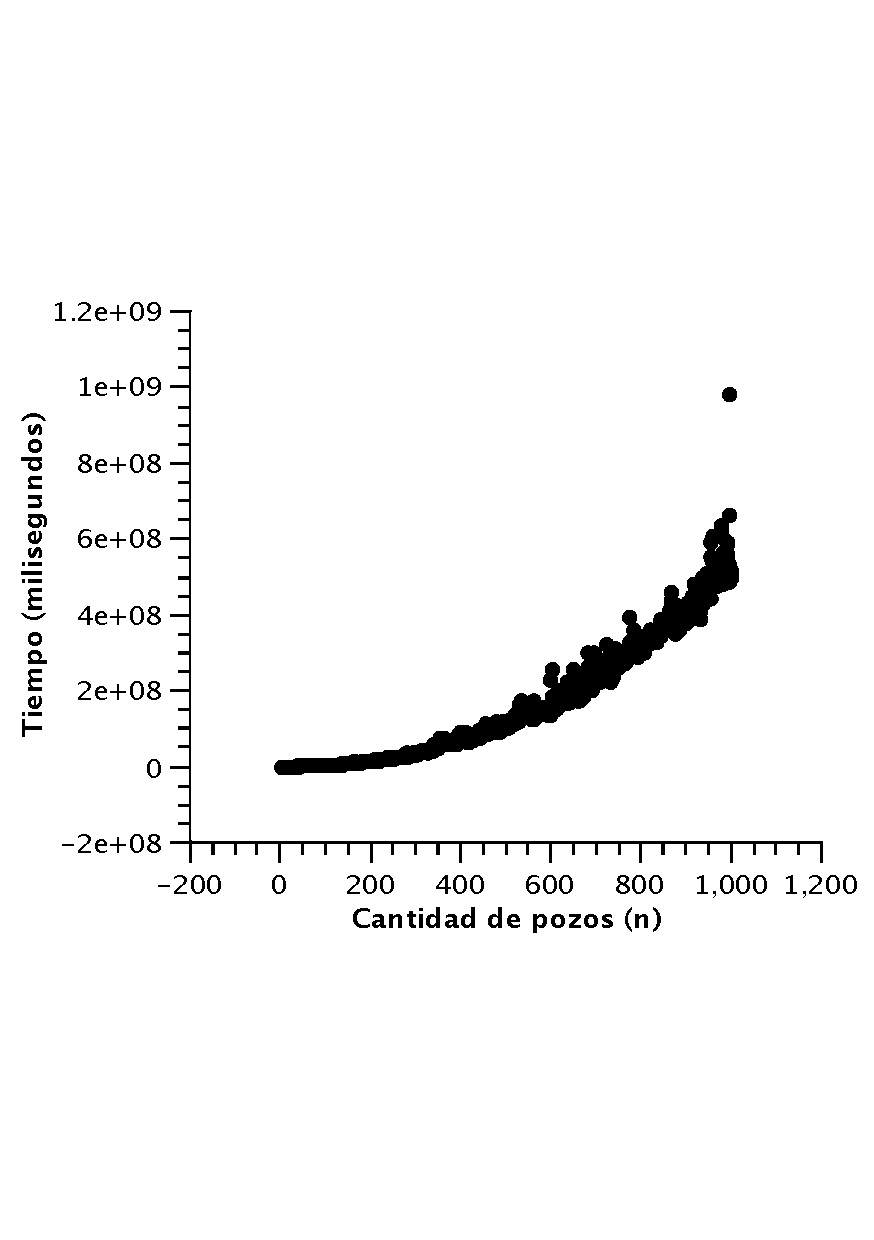
\includegraphics[width=\textwidth]{imagenes/ej3-peor.pdf}
                \caption{Tiempos sin procesar, en milisegundos}
        \end{subfigure}%

        \begin{subfigure}[b]{0.5\textwidth}
                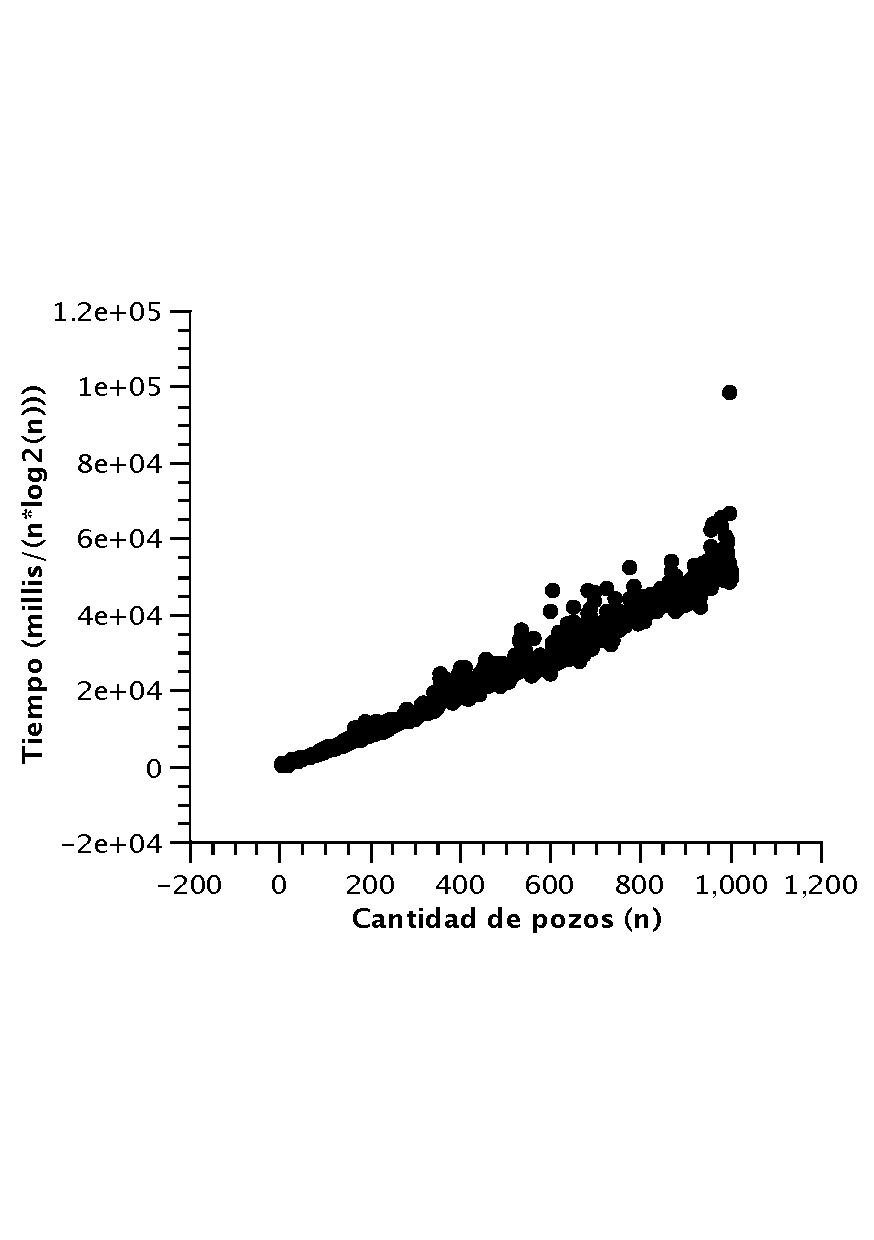
\includegraphics[width=\textwidth]{imagenes/ej3-peor-lineal.pdf}
                \caption{Dividiendo a los tiempos por $n \log(n)$}
        \end{subfigure}

\end{figure}

\begin{figure}[H]
        \centering

        \begin{subfigure}[b]{0.5\textwidth}
                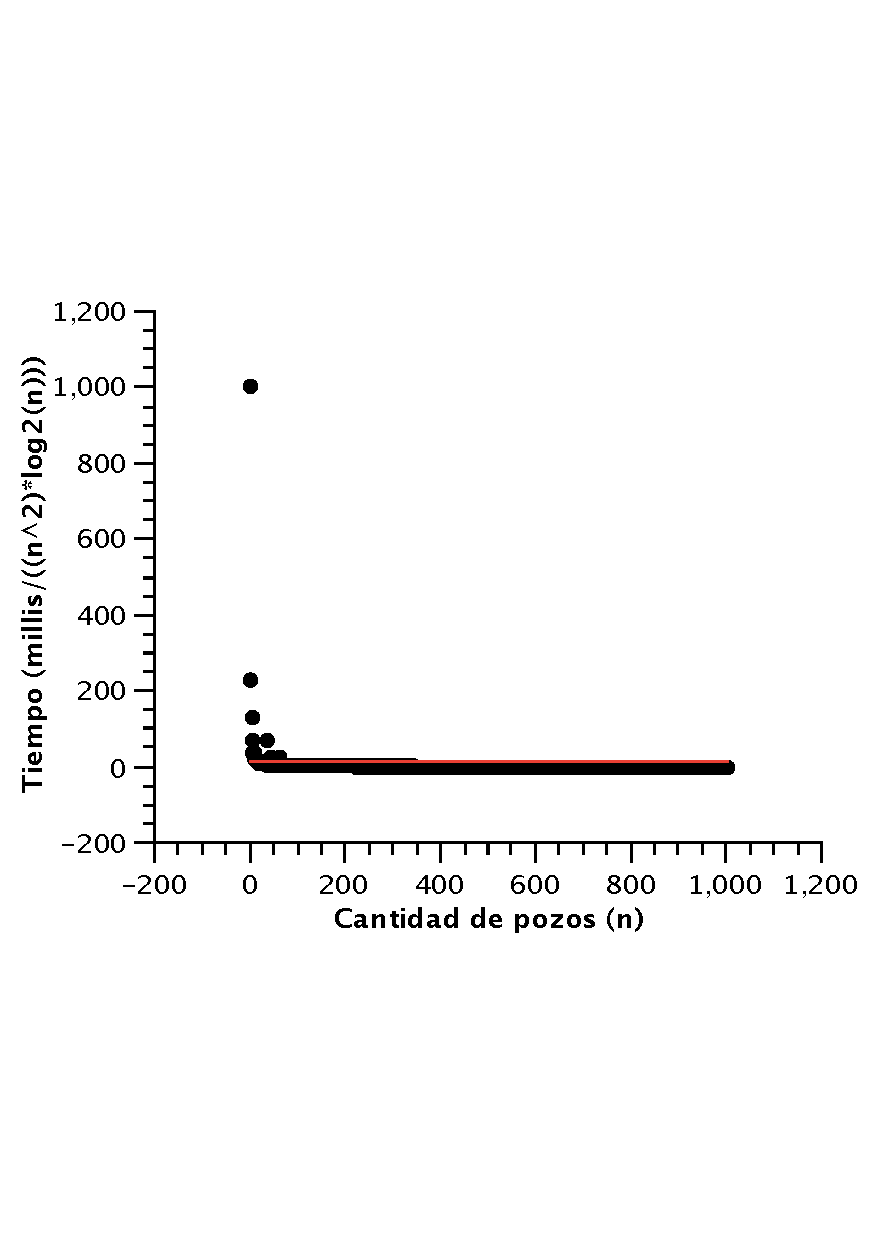
\includegraphics[width=\textwidth]{imagenes/ej3-peor-const.pdf}
                \caption{Dividiendo a los tiempos por $n^2 \log(n)$}
        \end{subfigure}

\end{figure}

A continuación, adjuntamos una tabla con los últimos 20 valores obtenidos en las instancias aleatorias, teniendo en cuenta que los casos fueron previamente ordenados según el tamaño ($n$):

\begin{table}[H]
\parbox{0.3\textwidth}{
    \begin{tabular}{ | l | l | l | l |}
    \hline
n   &Tiempo(milisegundos) &Tiempo(mili/($n^2 \log(n)$)) &Tiempo(mili/($n \log(n)$)))\\ \hline
980	&493,460,879.75	&50,674.23338154993	&0.08452622007433862\\ \hline
981	&482,018,120.4	&49,441.38037692552	&0.09101871660609798\\ \hline
982	&510,165,009.05	&52,267.43419346325	&0.08472145916999867\\ \hline
983	&516,396,402.7	&52,844.22546197011	&0.08947293513434787\\ \hline
984	&561,265,941.75	&57,369.01031618338	&0.07824592057934007\\ \hline
985	&490,971,048.75	&50,125.58045390238	&0.1026006503166199\\ \hline
986	&525,554,033.5	&53,594.01449803058	&0.09532040618344501\\ \hline
987	&570,880,765.55	&58,148.72977958777	&0.1056907440396239\\ \hline
988	&596,367,785.8	&60,674.39059893046	&0.08665430150997189\\ \hline
989	&566,389,457.35	&57,557.68953594214	&0.09656804009648187\\ \hline
990	&508,075,400.3	&51,571.981884774	&0.09234514821696686\\ \hline
991	&583,108,179.7	&59,119.77408159488	&0.1045670681684471\\ \hline
992	&587,978,851.1	&59,544.79875082848	&0.0944663358419995\\ \hline
993	&557,400,980.3	&56,383.08875465296	&0.1324639066988179\\ \hline
994	&590,795,854.55	&59,692.27032416804	&0.07456885483672317\\ \hline
995	&979,012,067	&98,802.68285405725	&0.1032966094149012\\ \hline
996	&662,148,109.4	&66,747.71182669644	&0.09686879345266487\\ \hline
997	&532,542,101.5	&53,621.16473927397	&0.1027177598861123\\ \hline
998	&525,905,149.05	&52,892.15775233119	&0.09732184303195211\\ \hline
999	&486,305,604.75	&48,853.44686677655	&0.1106853151800258\\ \hline
1,000	&497,043,395.25	&49,874.99037230599	&0.08448103791447331\\ \hline
    \end{tabular}
}
\end{table}

Como podemos ver de los gráficos y la tabla suministrada, al dividir los tiempos por $n* \log(n)$, tienden a algo lineal, mientras que al dividir los tiempos por $n^2* \log(n)$, tienden a un número constante. Entonces nuestro algoritmo tendría complejidad $\mathcal{O}(c*n^2* \log(n))$, donde $c$ es la constante a la cual converge el gráfico y esto se cumple incluso en el peor caso. Por lo tanto concluimos que los gráficos se condicen con nuestra predicción de complejidad. \\
\\

Por otro lado, una instancia de mejor caso sería una donde dado $n$, las tuberías posibles $m$ sean una cantidad aleatoria y que todas tengan costo mayor a $c$.

El detalle de intervalos es el siguiente:
\begin{itemize}
	\item Cantidad de pozos ($n$): 2 $\leq n \leq$ 1000
    \item Cantidad de tuberías ($m$): 1 $\leq m \leq \frac{n(n-1)}{2}$
    \item Costo de refinería ($c$): 2 $\leq c \leq$ 1000
\end{itemize}

No se generaron muestras para n = 1 ya que no hay tuberías posibles.
Generamos 20 instancias aleatorias para cada $n$, variando el $c$ en cada muestra pero fijando para toda tubería un costo mayor a $c-1$ en cada muestra y luego fueron promediadas. Su medición temporal, arroja el siguiente resultado:

\begin{figure}[H]
        \centering
\begin{subfigure}[b]{0.5\textwidth}
                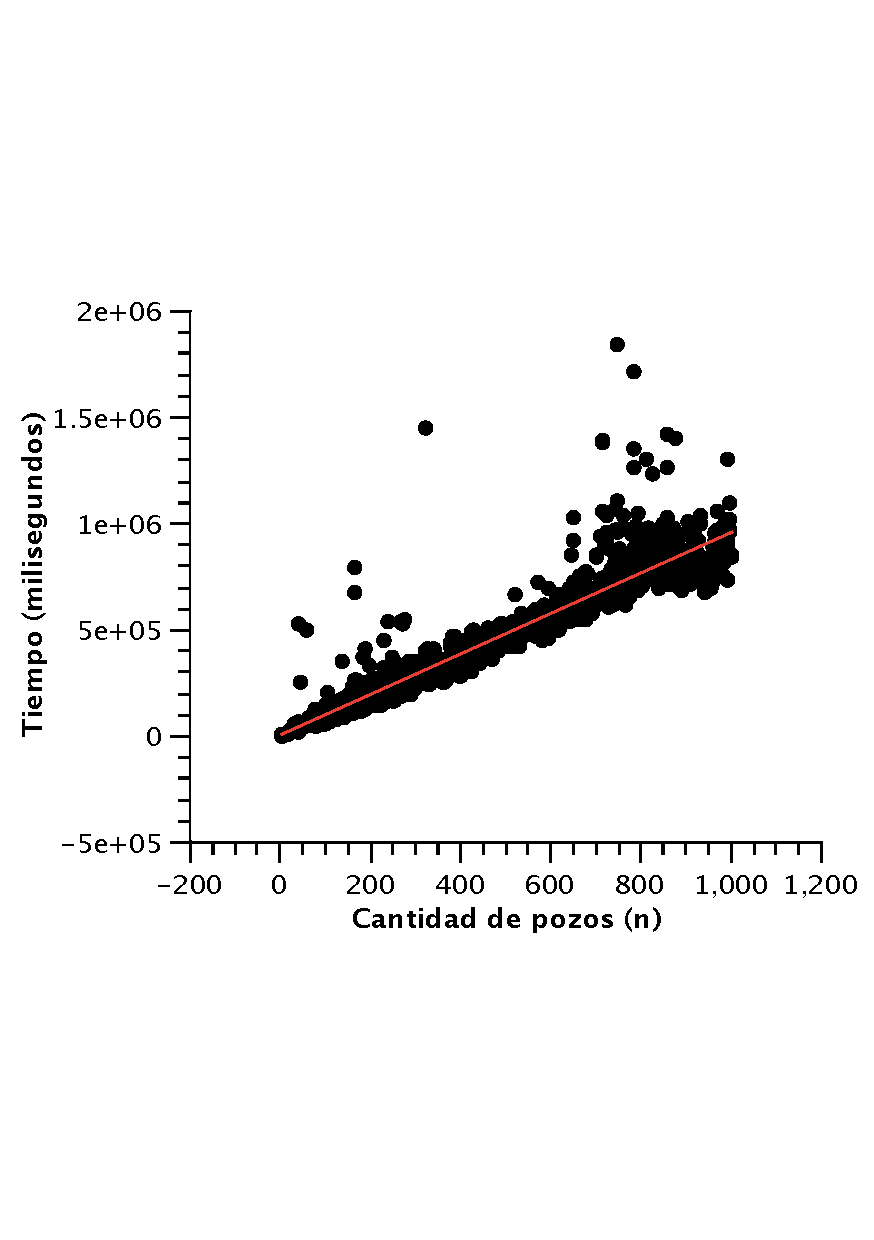
\includegraphics[width=\textwidth]{imagenes/ej3-mejor-lineal.pdf}
                \caption{Tiempos sin procesar, en milisegundos}
        \end{subfigure}%

        \begin{subfigure}[b]{0.5\textwidth}
                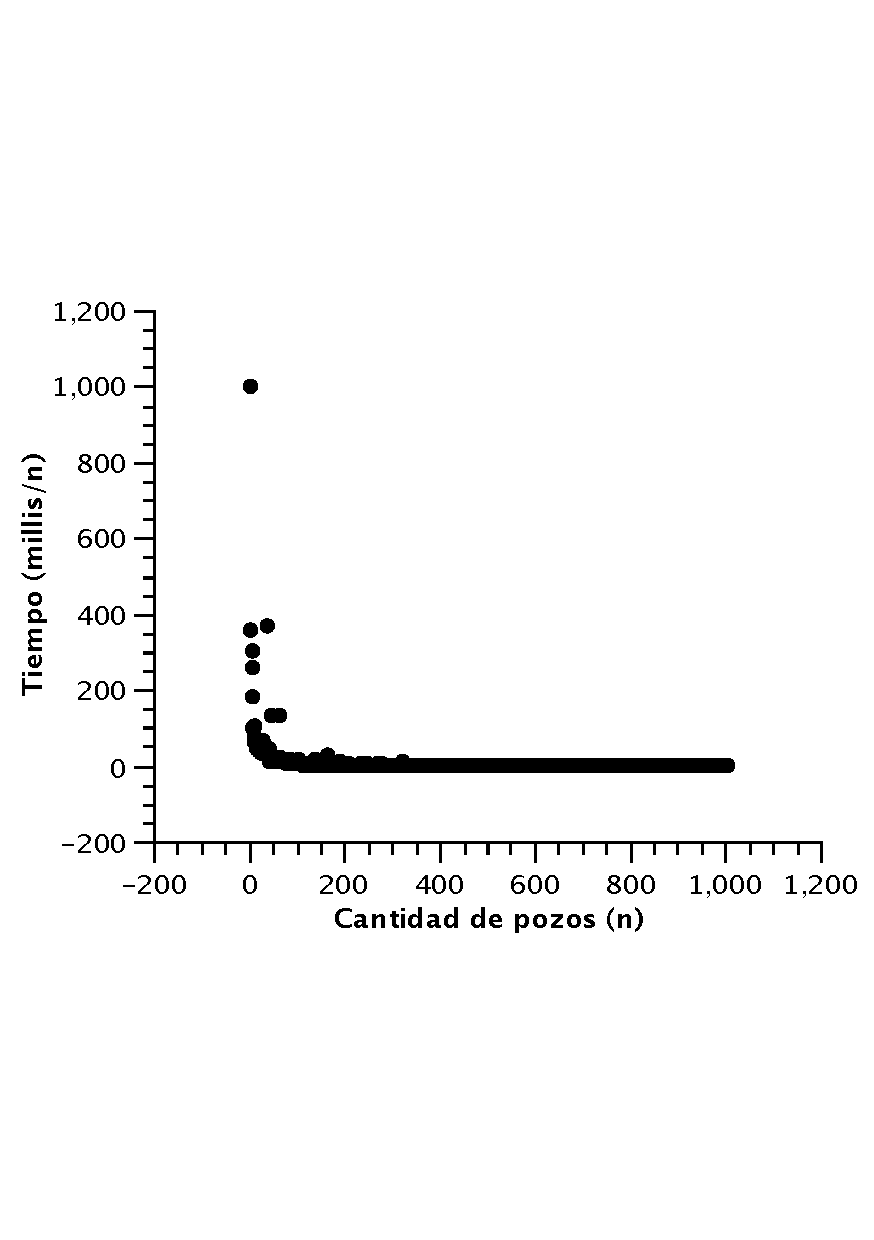
\includegraphics[width=\textwidth]{imagenes/ej3-mejor-const.pdf}
                \caption{Dividiendo a los tiempos por $n$}
        \end{subfigure}

\end{figure}

A continuación, adjuntamos una tabla con los últimos 20 valores obtenidos en las instancias aleatorias, teniendo en cuenta que los casos fueron previamente ordenados según el tamaño ($n$):

\begin{table}[H]
\parbox{0.3\textwidth}{
    \begin{tabular}{ | l | l | l |}
    \hline
n   &Tiempo(milisegundos) &Tiempo(mili/($n)$))\\ \hline
980	&806,646.15	&823.1083163265306\\ \hline
981	&870,507.45	&887.3674311926605\\ \hline
982	&812,053.05	&826.9379327902241\\ \hline
983	&859,470.3	&874.3339776195321\\ \hline
984	&753,265.6	&765.5138211382114\\ \hline
985	&989,880.6	&1,004.954923857868\\ \hline
986	&921,645.45	&934.7316937119675\\ \hline
987	&1,024,139.9	&1,037.629078014184\\ \hline
988	&841,503.3	&851.723987854251\\ \hline
989	&939,813.15	&950.2660768452984\\ \hline
990	&900,665.7	&909.7633333333333\\ \hline
991	&1,022,080.15	&1,031.362411705348\\ \hline
992	&925,351.25	&932.8137600806451\\ \hline
993	&1,300,366.2	&1,309.532930513595\\ \hline
994	&733,606.55	&738.0347585513078\\ \hline
995	&1,018,423.6	&1,023.541306532663\\ \hline
996	&957,110.3	&960.9541164658635\\ \hline
997	&1,017,087.7	&1,020.1481444333\\ \hline
998	&965,732.85	&967.6681863727455\\ \hline
999	&1,100,701.5	&1,101.803303303303\\ \hline
1,000	&841,919.8	&841.9198\\ \hline
1,001	&849,901	&849.0519480519481\\ \hline
\end{tabular}
}
\end{table}

Como podemos ver de los gráficos y la tabla suministrada, al dividir los tiempos por $n$, tienden a un número constante. Entonces nuestro algoritmo tendría complejidad $\mathcal{O}(c*n)$, donde $c$ es la constante a la cual converge el gráfico. Esto sucede porque como todas las tuberías tienen costo mayor a $c$, ninguna es añadida a la cola de prioridad, y por ende no es necesario solucionar el problema ya que la solución de menor costo es poner una refinería en cada pozo. El algoritmo es $\mathcal{O}(n)$ en mejor caso porque es lo que cuesta el ciclo que recorre el UnionFind para ver donde va una refinería, que en este caso es $\mathcal{O}(1)$ porque todas se tienen como raíz a si mismas.